\documentclass[border=6pt]{standalone}
\usepackage[T1]{fontenc}
\usepackage{lmodern}
\usepackage{amsmath,amssymb}
\usepackage{tikz}
\usetikzlibrary{positioning,arrows.meta,fit,calc}
\definecolor{wacvblue}{rgb}{0.21,0.49,0.74}
\hyphenpenalty=10000 \exhyphenpenalty=10000
\begin{document}
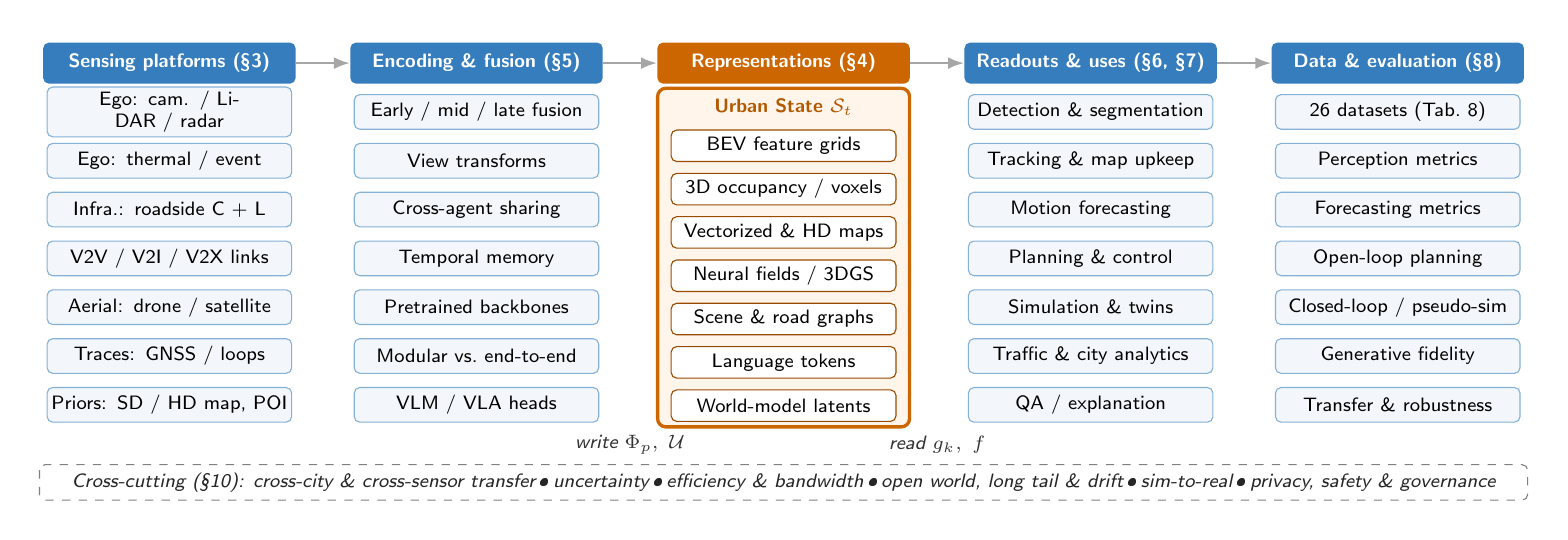
\begin{tikzpicture}[
  font=\sffamily\scriptsize,
  head/.style={rounded corners=2pt, fill=wacvblue, text=white, font=\sffamily\bfseries\scriptsize, text width=3.1cm, minimum height=0.52cm, align=center, inner sep=1.5pt},
  item/.style={rounded corners=2pt, draw=wacvblue!60, fill=wacvblue!6, text width=3.0cm, minimum height=0.44cm, align=center, inner sep=1.5pt},
  coreitem/.style={rounded corners=2pt, draw=orange!60!black, fill=white, text width=2.75cm, minimum height=0.4cm, align=center, inner sep=1.5pt},
  arr/.style={-{Latex[length=2mm]}, thick, gray!70}
]
\fill[white] (-1.8,0.45) rectangle (17.4,-5.7);
\def\xa{0} \def\xb{3.9} \def\xc{7.8} \def\xd{11.7} \def\xe{15.6}
\node[head] (h1) at (\xa,0) {Sensing platforms (\S3)};
\node[head] (h2) at (\xb,0) {Encoding \& fusion (\S5)};
\node[head, fill=orange!80!black] (h3) at (\xc,0) {Representations (\S4)};
\node[head] (h4) at (\xd,0) {Readouts \& uses (\S6, \S7)};
\node[head] (h5) at (\xe,0) {Data \& evaluation (\S8)};
\foreach \u/\v in {h1/h2,h2/h3,h3/h4,h4/h5} \draw[arr] (\u.east) -- (\v.west);
\foreach \t [count=\i] in {Ego: cam. / LiDAR / radar,Ego: thermal / event,Infra.: roadside C + L,V2V / V2I / V2X links,Aerial: drone / satellite,Traces: GNSS / loops,Priors: SD / HD map{,} POI}
  \node[item] at (\xa,-0.62*\i) {\t};
\foreach \t [count=\i] in {Early / mid / late fusion,View transforms,Cross-agent sharing,Temporal memory,Pretrained backbones,Modular vs.\ end-to-end,VLM / VLA heads}
  \node[item] at (\xb,-0.62*\i) {\t};
\draw[rounded corners=3pt, draw=orange!80!black, very thick, fill=orange!8] (\xc-1.6,-0.32) rectangle (\xc+1.6,-4.62);
\node[font=\sffamily\bfseries\scriptsize, orange!70!black] at (\xc,-0.56) {Urban State $\mathcal{S}_t$};
\foreach \t [count=\i] in {BEV feature grids,3D occupancy / voxels,Vectorized \& HD maps,Neural fields / 3DGS,Scene \& road graphs,Language tokens,World-model latents}
  \node[coreitem] at (\xc,-0.5-0.55*\i) {\t};
\foreach \t [count=\i] in {Detection \& segmentation,Tracking \& map upkeep,Motion forecasting,Planning \& control,Simulation \& twins,Traffic \& city analytics,QA / explanation}
  \node[item] at (\xd,-0.62*\i) {\t};
\foreach \t [count=\i] in {26 datasets (Tab.~8),Perception metrics,Forecasting metrics,Open-loop planning,Closed-loop / pseudo-sim,Generative fidelity,Transfer \& robustness}
  \node[item] at (\xe,-0.62*\i) {\t};
\node[font=\sffamily\scriptsize\itshape, gray!40!black] at ($(\xb,-4.85)!0.5!(\xc,-4.85)$) {write $\Phi_p,\ \mathcal{U}$};
\node[font=\sffamily\scriptsize\itshape, gray!40!black] at ($(\xc,-4.85)!0.5!(\xd,-4.85)$) {read $g_k,\ f$};
\draw[rounded corners=2pt, dashed, gray] (-1.65,-5.1) rectangle (17.25,-5.55);
\node[font=\sffamily\scriptsize\itshape, gray!30!black] at (7.8,-5.325) {Cross-cutting (\S10): cross-city \& cross-sensor transfer\,\textbullet\,uncertainty\,\textbullet\,efficiency \& bandwidth\,\textbullet\,open world, long tail \& drift\,\textbullet\,sim-to-real\,\textbullet\,privacy, safety \& governance};
\end{tikzpicture}
\end{document}
